\chapter{Interaction and bare vertex function}
\label{chapter:bare_vertex}

The interaction terms in the Hamiltonian can be divided into
intra- and inter-orbital terms,
\begin{equation}
H_{int}  =  H_{intra} + H_{inter}. 
\end{equation}
For the intra-orbital interactions we have the normal Hubbard $U$, i.e.
\begin{eqnarray}
H_{intra,\nu} & = & \sum_{\mathbf{r}} 
 U\, 
c^{\dagger}_{\mathbf{r}\nu\uparrow}
c_{\mathbf{r}\nu\uparrow}
c^{\dagger}_{\mathbf{r}\nu\downarrow} 
c_{\mathbf{r}\nu\downarrow} 
\\
& = & \sum_{\mathbf{r}} 
U\, 
c^{\dagger}_{\mathbf{r}\nu\uparrow}
c^{\dagger}_{\mathbf{r}\nu\downarrow}
c_{\mathbf{r}\nu\downarrow}
c_{\mathbf{r}\nu\uparrow}
\\
& = & \frac{1}{2} \sum_{\mathbf{r}\sigma,\mathbf{r}^{\prime}\sigma^{\prime}}
 V_{\nu\sigma\nu\sigma^{\prime}}(\mathbf{r},\mathbf{r}^{\prime}) 
c^{\dagger}_{\mathbf{r}\nu\sigma}
c^{\dagger}_{\mathbf{r}^{\prime}\nu\sigma^{\prime}}
c_{\mathbf{r}^{\prime}\nu\sigma^{\prime}}
c_{\mathbf{r}\nu\sigma}
\end{eqnarray}
where 
\begin{equation}
V_{\nu\sigma\nu\sigma^{\prime}}(\mathbf{r}, \mathbf{r}^{\prime} ) = 
\delta_{\mathbf{r},\mathbf{r}^{\prime}} \delta_{\sigma,-\sigma^{\prime}}\, U.
\end{equation}
Following, Abrikosov, Gorkov, and Dzyaloshinski, we rewrite
this as
\begin{equation}
H_{intra,\nu} = \frac{1}{2} \sum_{\mathbf{r}_1\sigma_1 \mathbf{r}_2 
\sigma_2 \sigma_3 \sigma_4}
 V_{\nu\sigma_1\nu\sigma_2,\nu\sigma_3\nu\sigma_4}(\mathbf{r}_1,\mathbf{r}_2) 
c^{\dagger}_{\mathbf{r}_1\nu\sigma_1}
c^{\dagger}_{\mathbf{r}_2\nu\sigma_2}
c_{\mathbf{r}_2\nu\sigma_4}
c_{\mathbf{r}_1\sigma_3}
\end{equation}
where
\begin{equation}
V_{\nu\sigma_1 \nu\sigma_2,\nu\sigma_3\nu\sigma_4}(\mathbf{r}_1, \mathbf{r}_2 ) = 
\delta_{\mathbf{r}_1,\mathbf{r}_2}\delta_{\sigma_1,\sigma_3} \delta_{\sigma_2,\sigma_4}
 \delta_{\sigma_1,-\sigma_2}\, U.
\end{equation}
Finally, we antisymmetrize the interaction to obtain the final
form
\begin{equation}
H_{intra,\nu} = \frac{1}{4} \sum_{\mathbf{r}_1\sigma_1
\mathbf{r}_2\sigma_2 \mathbf{r}_3\sigma_3 \mathbf{r}_4\sigma_4}
 \Gamma^{(0)}_{\nu\sigma_1\nu\sigma_2,\nu\sigma_3\nu\sigma_4}(\mathbf{r}_1, \mathbf{r}_2; 
\mathbf{r}_3, \mathbf{r}_4) 
\,c^{\dagger}_{\mathbf{r}_1\nu\sigma_1}
c^{\dagger}_{\mathbf{r}_2 \nu\sigma_2}
c_{\mathbf{r}_4\nu\sigma_4}
c_{\mathbf{r}_3 \nu \sigma_3}
\end{equation}
where
\begin{equation}
 \Gamma^{(0)}_{\nu\sigma_1\nu\sigma_2,\nu\sigma_3\nu\sigma_4}(\mathbf{r}_1 \mathbf{r}_2; 
\mathbf{r}_3, \mathbf{r}_4)
 = U\, \delta_{\mathbf{r}_1,\mathbf{r}_2} \delta_{\mathbf{r}_3,\mathbf{r}_1} 
\delta_{\mathbf{r}_4,\mathbf{r}_2}
\delta_{\sigma_1,-\sigma_2}
\left(\delta_{\sigma_1,\sigma_3} \delta_{\sigma_2,\sigma_4}
 - \delta_{\sigma_1,\sigma_4} \delta_{\sigma_2,\sigma_3}\right).
\end{equation}
and the diagramatic representation of
the vertex function is as below.\\
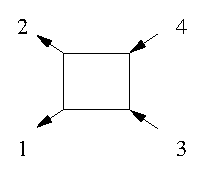
\epsfig{file=model/bare_vertex.eps}\\
Note that it may also be convenient to use the symmetric form
of the vertex function,
\begin{equation}
\Gamma^{(0)}_{\nu\sigma_1\nu\sigma_2,\nu\sigma_3\nu\sigma_4}(\mathbf{r}_1, \mathbf{r}_2; 
\mathbf{r}_3, \mathbf{r}_4)
 = \frac{U}{2}\, \delta_{\mathbf{r}_1,\mathbf{r}_2} 
\delta_{\mathbf{r}_3,\mathbf{r}_1} \delta_{\mathbf{r}_4,\mathbf{r}_2}
\left( \delta_{\sigma_1,\sigma_3}\delta_{\sigma_2,\sigma_4}
 - \vec{\sigma}_{\sigma_1,\sigma_3}\cdot
 \vec{\sigma}_{\sigma_2,\sigma_4} \right).
\end{equation}

Note that the vertex function is non-zero only in 
certain special cases:
\begin{eqnarray}
\sigma_1 = \sigma_3,\;\sigma_2 = \sigma_4 = -\sigma_1 & \to &
\Gamma^{(0)} = U \\
\sigma_1 = \sigma_4, \;\sigma_2 = \sigma_3 = -\sigma_1 & \to &
\Gamma^{(0)} = -U
\end{eqnarray}

In the Nambu representation we need to expand the vertex
to properly account for the mixed particle-hole basis
for the creation and annihilation operators.  If,
as before, we define
\begin{eqnarray}
\psi_{\mathbf{r}\nu 0} & = & c_{\mathbf{r}\nu\uparrow} \\   
\psi_{\mathbf{r}\nu 1} & = & c_{\mathbf{r}\nu\downarrow} \\
\psi_{\mathbf{r}\nu 2} & = & c^{\dagger}_{\mathbf{r}\nu\uparrow} \\
\psi_{\mathbf{r}\nu 3} & = & c^{\dagger}_{\mathbf{r}\nu\downarrow},
\end{eqnarray}
then we have additional terms in a vertex function
which is symmetrized within the particle-hole space.
All terms in the fully-symmetrized vertex can be represented
by the following vertex diagram for 
$\Gamma^{(0)}_{\nu\alpha_1\nu\alpha_2;\nu\alpha_3\nu\alpha_4}:$ \\
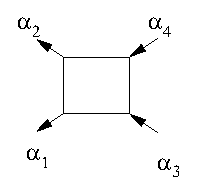
\epsfig{file=model/bare_vertex_mod.eps}\\

Here we show the relations for generalizing the vertex to
the expanded space.  Let $\overline{\alpha}$ represent
the operators that orginate from the expanded space, \textit{i.e.}
$\overline{c_{\uparrow}} = c^{\dagger}_{\uparrow}$.
\begin{eqnarray}
\Gamma^{(0)}_{\overline{1}2;\overline{3}4}
\psi^{\dagger}_{\overline{1}}\psi^{\dagger}_2
\psi_4 \psi_{\overline{3}}
& \equiv & 
\Gamma^{(0)}_{\overline{1}2;\overline{3}4}
\psi_1 \psi^{\dagger}_2
\psi_4 \psi^{\dagger}_3 \\
& = & -\Gamma^{(0)}_{\overline{1}2;\overline{3}4}
\psi^{\dagger}_2\psi_1 \psi_4 \psi^{\dagger}_3 \\
& = & -\Gamma^{(0)}_{\overline{1}2;\overline{3}4}
\psi^{\dagger}_2\psi^{\dagger}_3 \psi_1 \psi_4 \\
& \equiv & \Gamma^{(0)}_{23;41}\psi^{\dagger}_2\psi^{\dagger}_3 \psi_1 \psi_4 
\end{eqnarray}
From which we get
\begin{equation}
\Gamma^{(0)}_{\overline{1}2;\overline{3}4} = -\Gamma^{(0)}_{23;41}.
\end{equation}
\begin{eqnarray}
\Gamma^{(0)}_{1\overline{2};3\overline{4}}
\psi^{\dagger}_{1}\psi^{\dagger}_{\overline{2}}
\psi_{\overline{4}} \psi_3 \\
& = & \Gamma^{(0)}_{1\overline{2};3\overline{4}}
\psi^{\dagger}_{1}\psi_{2}
\psi^{\dagger}_{4} \psi_3 \\
& = & - \Gamma^{(0)}_{1\overline{2};3\overline{4}}
\psi^{\dagger}_{1}\psi^{\dagger}_{4}
\psi_{2} \psi_3 \\
& \equiv & \Gamma^{(0)}_{14;32}
\psi^{\dagger}_{1}\psi^{\dagger}_{4}
\psi_{2} \psi_3 \\
\end{eqnarray}
From which we get
\begin{equation}
\Gamma^{(0)}_{1\overline{2};3\overline{4}} = -\Gamma^{(0)}_{14;32}.
\end{equation}
\begin{eqnarray}
\Gamma^{(0)}_{1\overline{2};\overline{3}4}
\psi^{\dagger}_{1}\psi^{\dagger}_{\overline{2}}
\psi_4 \psi_{\overline{3}} \\
& \equiv & \Gamma^{(0)}_{1\overline{2};\overline{3}4}
\psi^{\dagger}_1\psi_2
\psi_4 \psi^{\dagger}_3 \\
& = & \Gamma^{(0)}_{1\overline{2};\overline{3}4}
\psi^{\dagger}_1\psi^{\dagger}_3
\psi_2 \psi_4 \\
& \equiv & \Gamma^{(0)}_{1 3; 4 2}
\psi^{\dagger}_1\psi^{\dagger}_3
\psi_2 \psi_4 
\end{eqnarray}
From which we get
\begin{equation}
\Gamma^{(0)}_{1\overline{2};\overline{3}4}
= \Gamma^{(0)}_{1 3; 4 2}
\end{equation}
\begin{eqnarray}
\Gamma^{(0)}_{\overline{1}2;3\overline{4}}
\psi^{\dagger}_{\overline{1}}\psi^{\dagger}_2
\psi_{\overline{4}} \psi_3 
&  \equiv &
\Gamma^{(0)}_{\overline{1}2;3\overline{4}}
\psi_1\psi^{\dagger}_2
\psi^{\dagger}_4 \psi_3  \\
& = & \Gamma^{(0)}_{\overline{1}2;3\overline{4}}
\psi^{\dagger}_2\psi^{\dagger}_4\psi_1\psi_3 \\
& \equiv & \Gamma^{(0)}_{24;31}
\psi^{\dagger}_2\psi^{\dagger}_4\psi_1\psi_3
\end{eqnarray}
from which we get
\begin{equation}
\Gamma^{(0)}_{\overline{1}2;3\overline{4}} =
\Gamma^{(0)}_{24;31}.
\end{equation}
Finally, we have
\begin{eqnarray}
\Gamma^{(0)}_{\overline{1}\overline{2};\overline{3}\overline{4}}
\psi^{\dagger}_{\overline{1}}\psi^{\dagger}_{\overline{2}}
\psi_{\overline{4}} \psi_{\overline{3}} 
&  \equiv &
\Gamma^{(0)}_{\overline{1}\overline{2};\overline{3}\overline{4}}
\psi_1\psi_2
\psi^{\dagger}_4 \psi^{\dagger}_3  \\
& = &
\Gamma^{(0)}_{\overline{1}\overline{2};\overline{3}\overline{4}}
\psi^{\dagger}_4 \psi^{\dagger}_3 \psi_1\psi_2 \\
& \equiv &
\Gamma^{(0)}_{4 3; 2 1} \psi^{\dagger}_4 \psi^{\dagger}_3 \psi_1\psi_2
\end{eqnarray}
from which we get
\begin{equation}
\Gamma^{(0)}_{\overline{1}\overline{2};\overline{3}\overline{4}} =
\Gamma^{(0)}_{4 3; 2 1}.
\end{equation}

For the single-band Hubbard model, the above produces
the following:
\begin{eqnarray}
\Gamma^{(0)}_{01;01} & = U  \;\;\;\; & \Gamma^{(0)}_{01;10} = -U \\
\Gamma^{(0)}_{03;03} & = -U \;\;\;\; & \Gamma^{(0)}_{03;30} = U \\
\Gamma^{(0)}_{02;13} & = U \;\;\;\; & \Gamma^{(0)}_{02;31} = -U \\
\\
\Gamma^{(0)}_{10;10} & = U \;\;\;\; & \Gamma^{(0)}_{10;01} = -U \\
\Gamma^{(0)}_{12;12} & = -U \;\;\;\; & \Gamma^{(0)}_{12;21} = U \\
\Gamma^{(0)}_{13;02} & = U \;\;\;\; & \Gamma^{(0)}_{13;20} = -U \\
\\
\Gamma^{(0)}_{23;23} & = U \;\;\;\; & \Gamma^{(0)}_{23;32} = -U \\
\Gamma^{(0)}_{21;21} & = -U \;\;\;\; & \Gamma^{(0)}_{21;12} = U \\
\Gamma^{(0)}_{20;31} & = U \;\;\;\; & \Gamma^{(0)}_{20;13} = -U \\
\\
\Gamma^{(0)}_{32;32} & = U \;\;\;\; & \Gamma^{(0)}_{32;23} = -U \\
\Gamma^{(0)}_{30;30} & = -U  \;\;\;\; & \Gamma^{(0)}_{30;03} = U \\
\Gamma^{(0)}_{31;20} & = U \;\;\;\; & \Gamma^{(0)}_{31;02} = -U 
\end{eqnarray}
